\begin{frame}{Aplicações}{Reconhecimento Automático de Placas}

\begin{figure}
    \centering
    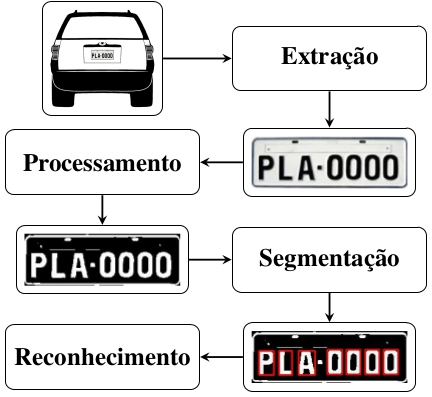
\includegraphics[scale=.4]{img/lpr.jpeg}
    \caption{Etapas gerais de um processo de RAP. (Fonte: Autoral)}
    \label{fig:lpr_recognition}
\end{figure}

\end{frame}

\begin{frame}{Aplicações}{Reconhecimento de Faces (Expressões)}

\begin{figure}
    \centering
    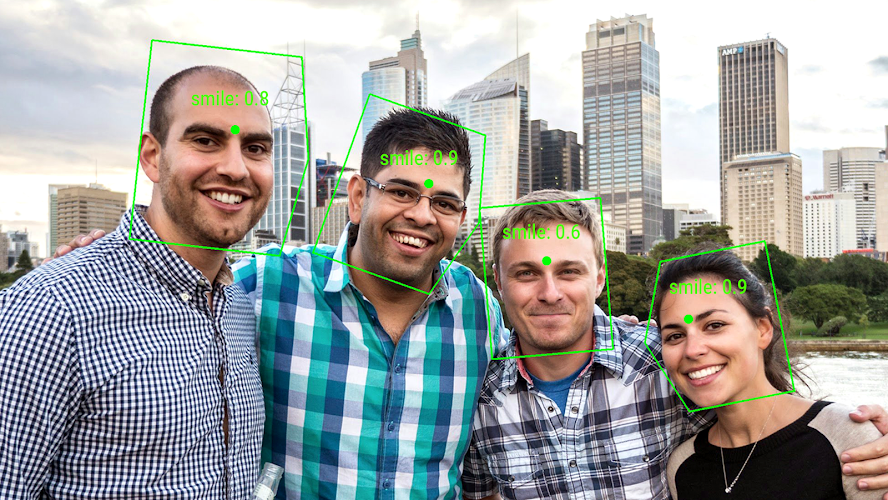
\includegraphics[scale=.3]{img/face_recognition.png}
    \caption{Reconhecimento de faces e de expressões. (Fonte: Mobile Vision - https://developers.google.com/vision/)}
    \label{fig:face_recognition}
\end{figure}

\end{frame}

\begin{frame}{Aplicações}{Reconhecimento de gestos}

\begin{figure}
    \centering
    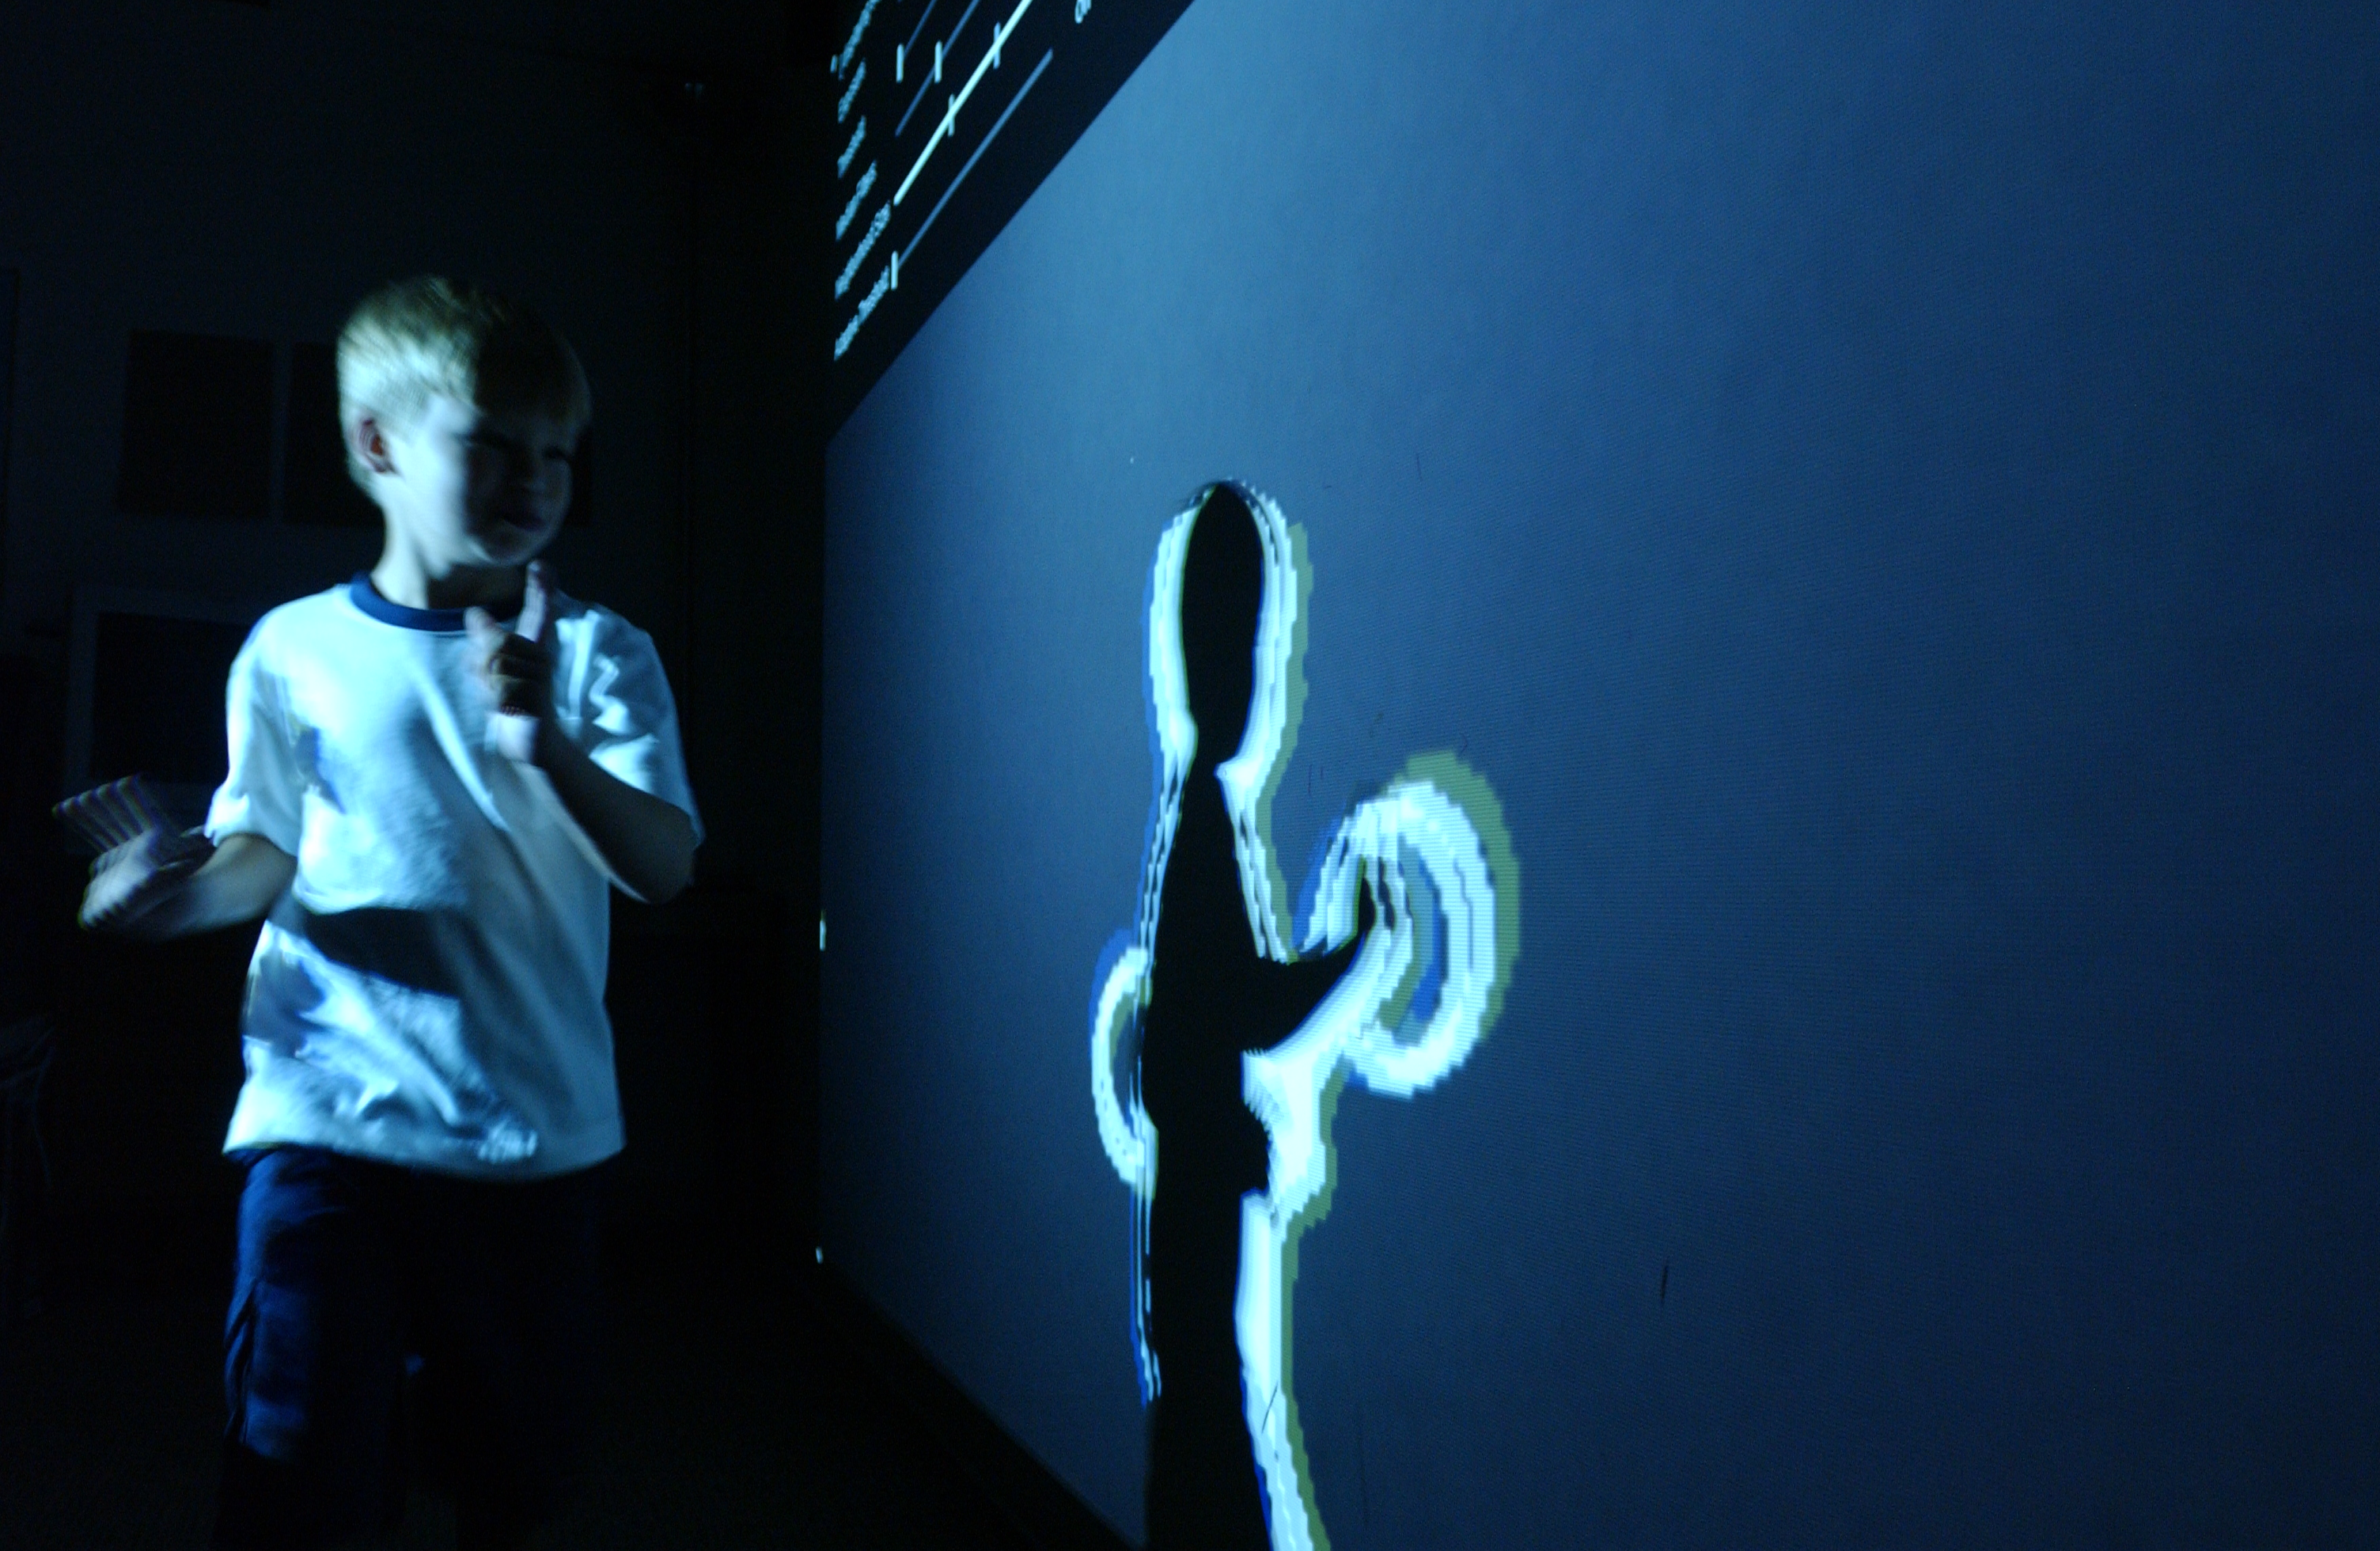
\includegraphics[scale=.4]{img/gesture_recognition.jpg}
    \caption{(Fonte: Wikipedia - https://en.wikipedia.org/ \\ wiki/Gesture\_recognition)}
    \label{fig:gesture_recognition}
\end{figure}

\end{frame}

\begin{frame}{Aplicações}{Veículos Autônomos}

\begin{figure}
    \centering
    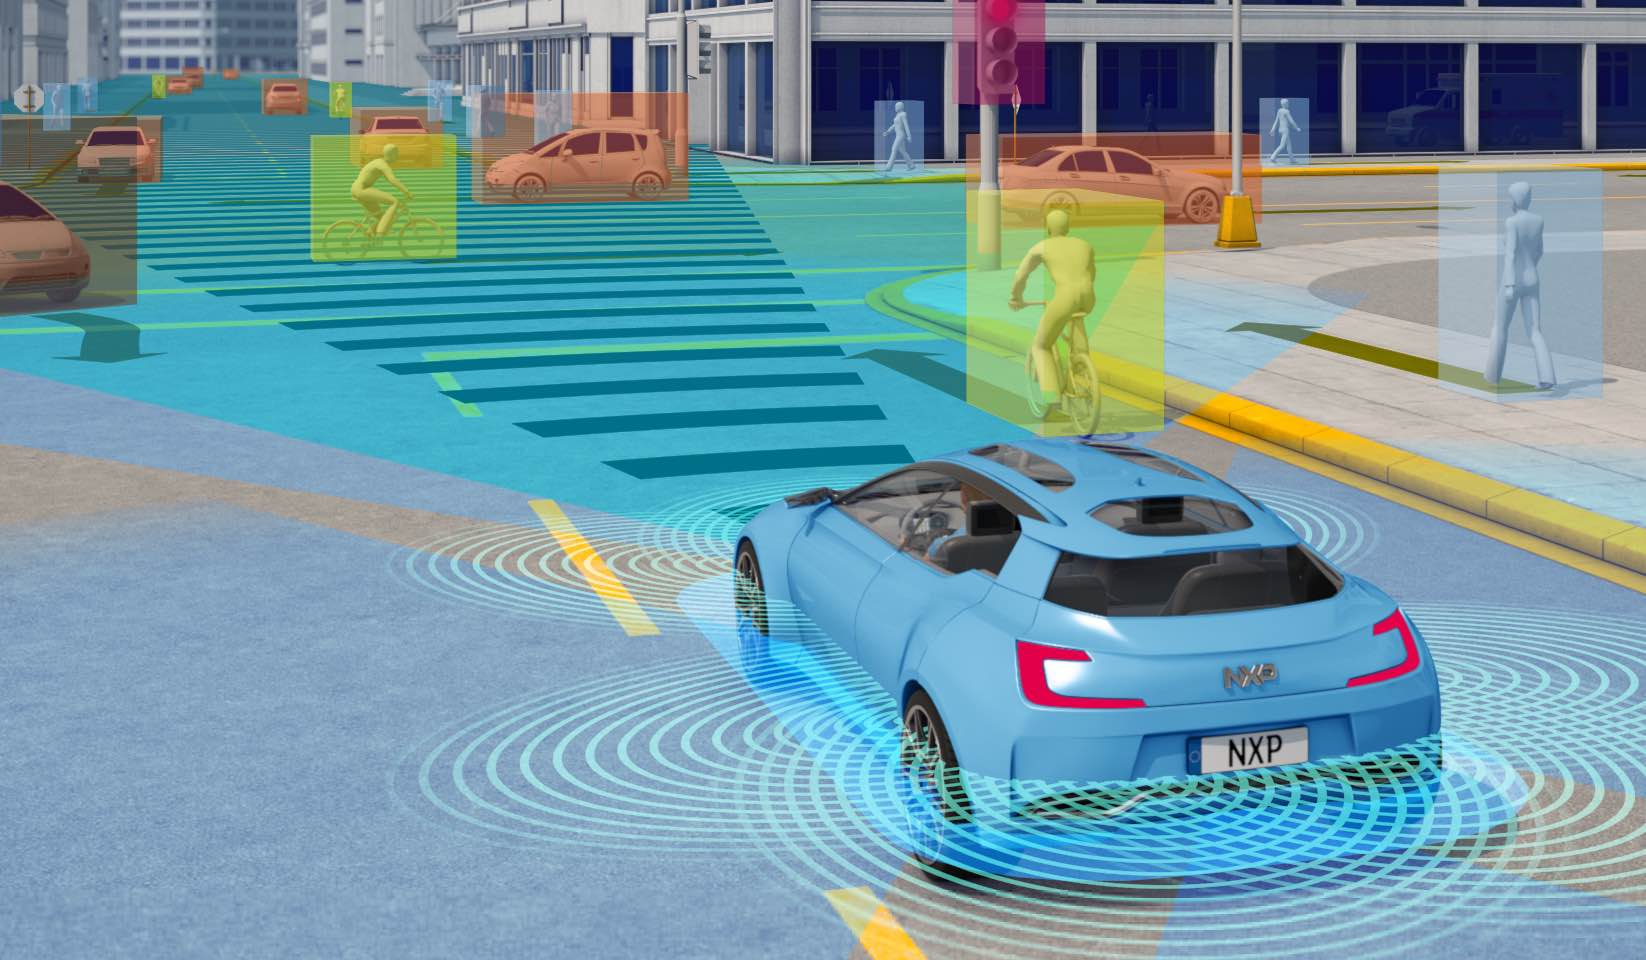
\includegraphics[scale=.18]{img/autonomous_car.jpg}
    \caption{(Fonte: Electronics Weekly - https://www.electronicsweekly.com/market-sectors/automotive-electronics/ces-autonomous-cars-sensors-make-safe-2017-01/)}
    \label{fig:gesture_recognition}
\end{figure}

\end{frame}

\begin{frame}{Aplicações}{Coleções de Fotos Pessoais}

\begin{figure}
    \centering
    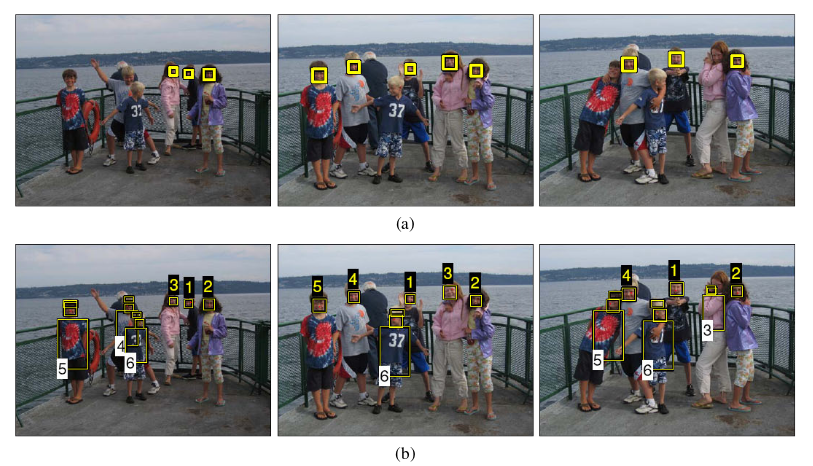
\includegraphics[scale=.3]{img/personal_collection.png}
    \caption{(Fonte: Computer Vision - Algorithms and Applications - Richard Szeliski)}
    \label{fig:personal_collection}
\end{figure}

\end{frame}

\begin{frame}{Aplicações}{Reconhecimento de Locais}

\begin{figure}
    \centering
    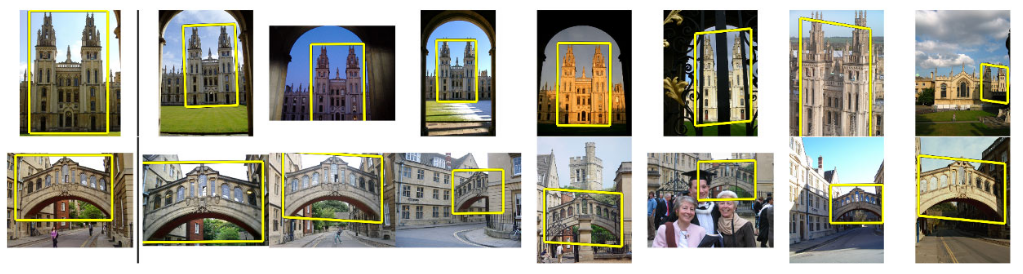
\includegraphics[scale=.3]{img/location_recognition.png}
    \caption{(Fonte: Computer Vision - Algorithms and Applications - Richard Szeliski)}
    \label{fig:location_recognition}
\end{figure}

\end{frame}

\begin{frame}{Aplicações}{Edições Inteligentes}

\begin{figure}
    \centering
    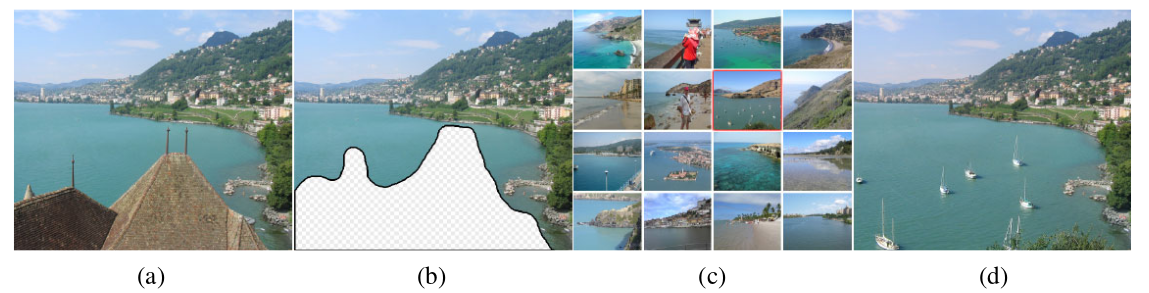
\includegraphics[scale=.28]{img/smart_editing.png}
    \caption{(Fonte: Computer Vision - Algorithms and Applications - Richard Szeliski)}
    \label{fig:smart_editing}
\end{figure}

\end{frame}

\begin{frame}{Aplicações}{Segmentação de Imagens Médicas}

\begin{figure}
    \centering
    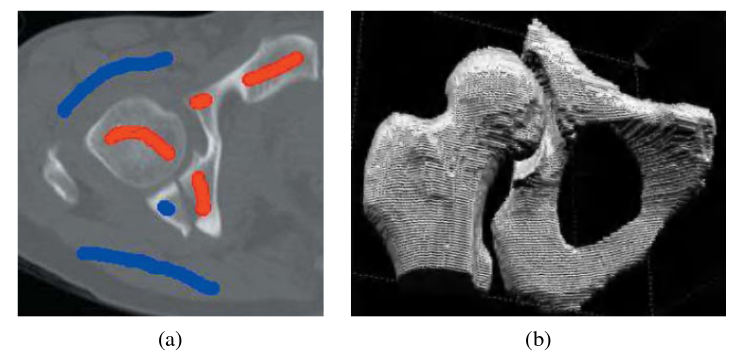
\includegraphics[scale=.4]{img/medical_image_segmentation.png}
    \caption{(Fonte: Computer Vision - Algorithms and Applications - Richard Szeliski)}
    \label{fig:medical_image_segmentation}
\end{figure}

\end{frame}

\begin{frame}{Aplicações}{Rastreamento de Contorno e Rotoscopia}

\begin{figure}
    \centering
    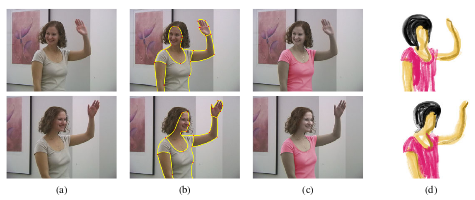
\includegraphics[scale=.6]{img/contour_trackin_rotoscoping.png}
    \caption{(Fonte: Computer Vision - Algorithms and Applications - Richard Szeliski)}
    \label{fig:contour_tracking_rotoscoping}
\end{figure}

\end{frame}

\begin{frame}{Aplicações}{Reconhecimento Ótico de Braille}

\begin{figure}
    \centering
    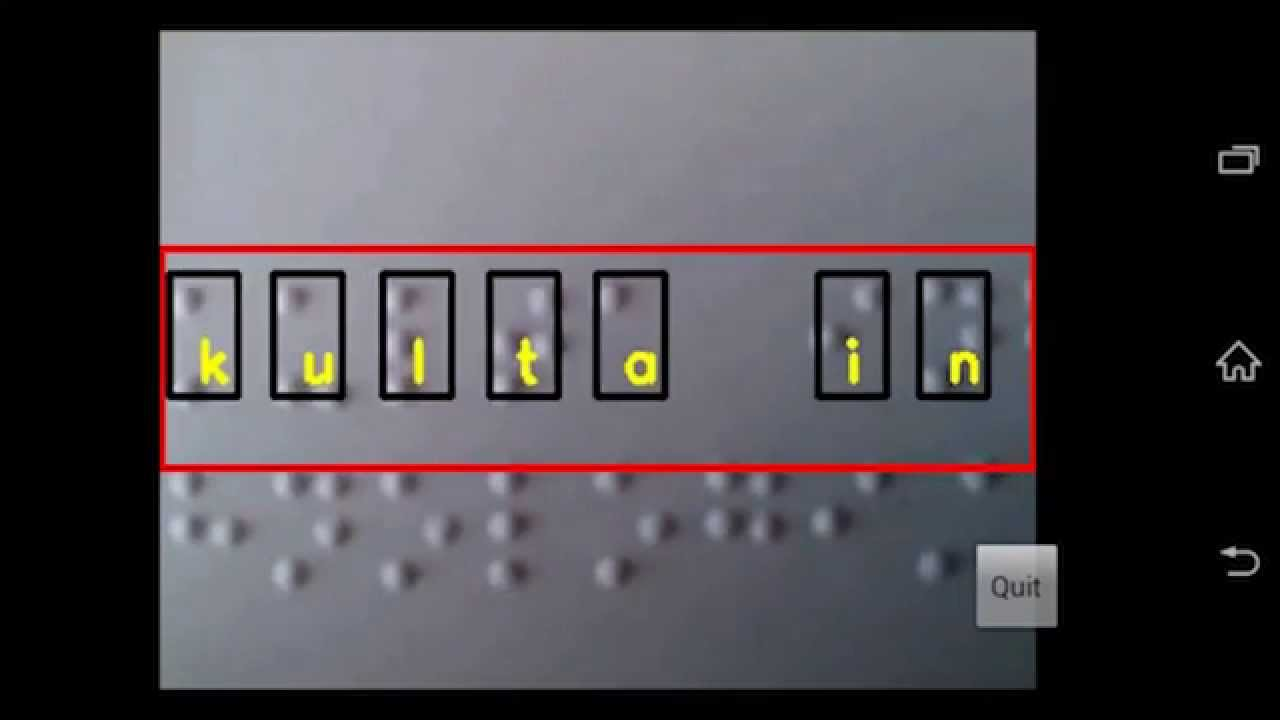
\includegraphics[scale=.2]{img/obr.jpg}
    \caption{(Fonte: Youtube - https://www.youtube.com/watch?v=X5kFdUsCkEA)}
    \label{fig:optical_braille_recognition}
\end{figure}

\end{frame}

\begin{frame}{Aplicações}{Reconhecimento de Impressões Digitais}

\begin{figure}

    \centering
    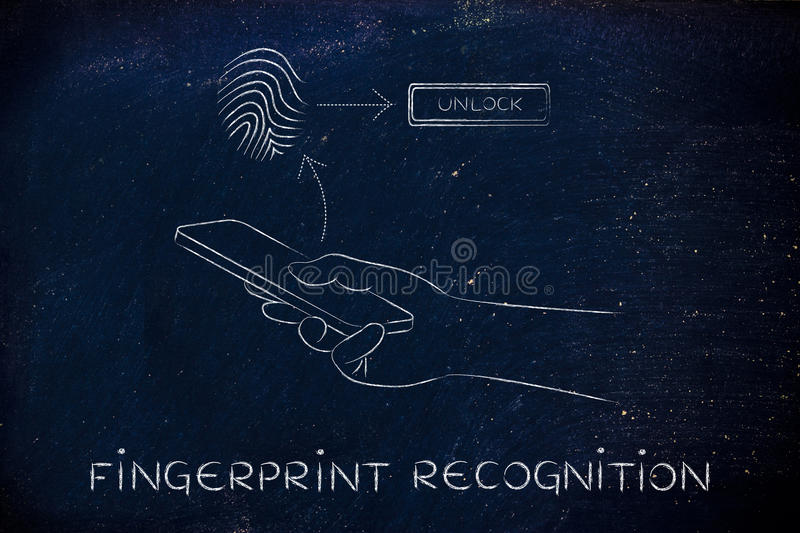
\includegraphics[scale=1]{img/fingerprint_recognition.jpg}
    \caption{(Fonte: Dreamstime - https://thumbs.dreamstime.com/b/fingerprint-recognition-smartphones-smartphone-user-touching-screen-to-unlock-68633965.jpg)}
    \label{fig:fingerprint_recognition}
\end{figure}

\end{frame} 

\begin{frame}{Aplicações}{Reconhecimento de Iris}

\begin{figure}

    \centering
    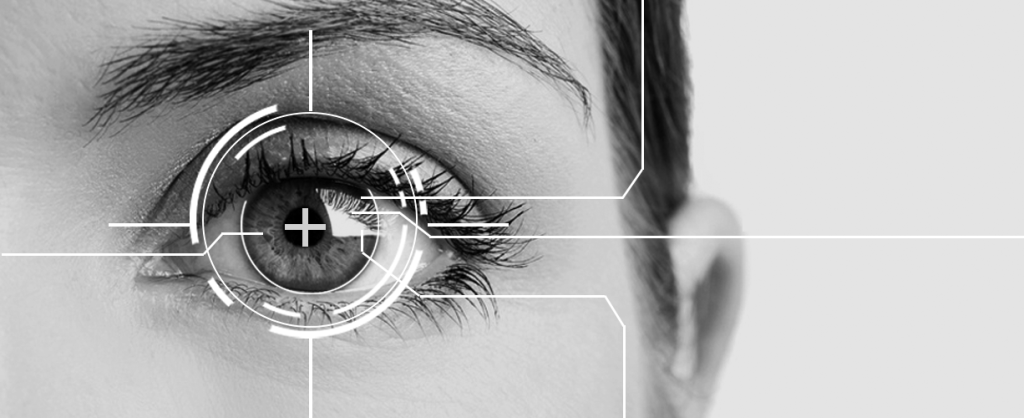
\includegraphics[scale=.3]{img/iris_recognition.png}
    \caption{(Fonte: Iritech - http://www.iritech.com/blog/iris-biometric-safe/)}
    \label{fig:iris_recognition}
\end{figure}

\end{frame}
